\lstset{
 showspaces=false,
 showtabs=false,
 frame=none,
 tabsize=2,
 breaklines=true,
 numbers=none,
 showstringspaces=false,
 breakatwhitespace=true,
 escapeinside={(*@}{@*)},
 keywordstyle=\bfseries,
 basicstyle=\footnotesize\ttfamily,
}

\section*{Lab activity 2}

\subsection*{Topology diagram}
\begin{figure}[htb]
	\centering
	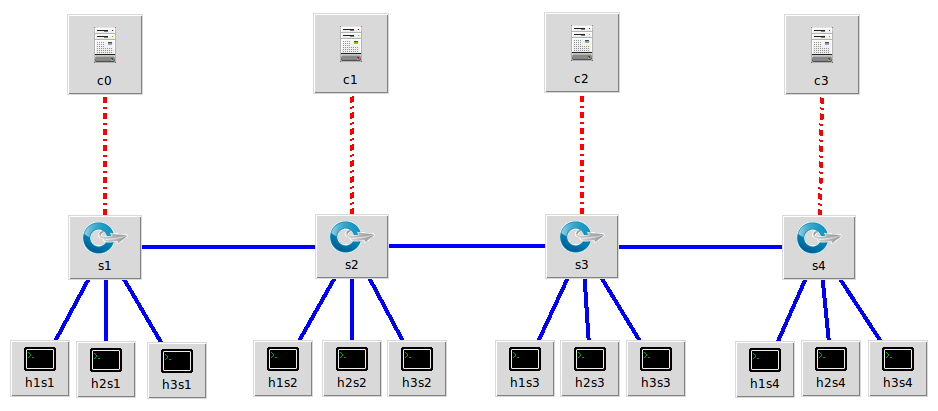
\includegraphics[width=1\linewidth]{img/topology-2.png}
	\caption{the topology that will be implemented during this lab activity.
  It is a linear topology with four switches connected to each other,
  each one connected to three hosts. Each switch is linked to a different
  SDN controller.}
	\label{fig:topology-2}
\end{figure}

\subsection*{Learning objectives}
After finishing this lab activity you will be able to:
\begin{itemize}
  \item Create a custom switch class that extends the OVSSwitch class provided
  by the Mininet Python API.
  \item Implement a cluster of local controllers inside Mininet using a custom
  switch class and the topology classes provided by the Mininet high-level API.
  \item Reflect on the reasons for implementing a cluster of local controllers
  using the topology templates provided by the high-level API instead of
  using the way shown in Activity 1.
  \item Test the network connectivity and the performance of a network with multiple
  local controllers.
\end{itemize}






\subsection*{Scenario}
In this activity you will implement the topology shown in figure \ref{fig:topology-2} using
a Python script and the classes provided by the high-level Mininet API, which
represent topology templates. In order to use these classes for creating a network
with multiple contollers, you will have to define a new switch class that extends
the OVSSwitch class normally used.

Begin by creating a new Python script, then import the Mininet classes required for
this activity. Create all the controllers required by the topology and define
the custom switch class which extends the class \code{OVSSwitch}. Define a new funcion for creating
the network and inside its body use one of the topology templates provided
by the Mininet API to implement the required topology.
After writing the script, execute it and test the network connectivity and its
performance.

This lab activity assumes that:
\begin{itemize}
  \item you are proficient in SDN networks
  \item you are proficient in Mininet network emulator
  \item you have a basic knowledge of the Python programming language
  \item you have completed Activity 1.
\end{itemize}






\subsection*{Task 1: create the controllers}
\subsubsection*{Step 1}
Create a new Python script and edit with the text editor you prefer. If you're editing
it inside the Mininet virtual machine, it is suggested to use Vim text editor.

\subsubsection*{Step 2}
Import the required Python classes from the Mininet API:
\begin{lstlisting}
#!/usr/bin/Python
from mininet.net import Mininet
from mininet.node import OVSSwitch, Controller
from mininet.topo import LinearTopo
from mininet.log import setLogLevel
from mininet.cli import CLI
\end{lstlisting}

\subsubsection*{Step 3}
Create the four required controllers, specifying for each one a different name and
a different TCP port:
\begin{lstlisting}
c0 = Controller( 'c0', port=6633 )
c1 = Controller( 'c1', port=6634 )
c2 = Controller( 'c2', port=6635 )
c3 = Controller( 'c3', port=6636 )
\end{lstlisting}

\subsubsection*{Step 4}
Create a new array and initialize it with the four created controllers:
\begin{lstlisting}
controllers = [c0, c1, c2, c3]
\end{lstlisting}
This array will be used later in the script to easily add all the controllers
to the network using a for loop (see Step 4 of Task 3).

\subsubsection*{Step 5}
Create a map that associates each switch to the relative controller:
\begin{lstlisting}
cmap = { 's1': c0, 's2': c1, 's3': c2, 's4' : c3 }
\end{lstlisting}






\subsection*{Task 2: create a custom switch class}
\subsubsection*{Step 1}
Define a new class called \code{MultiSwitch} wich extends the class
\code{OVSSwitch} provided by the Mininet API:
\begin{lstlisting}
class MultiSwitch( OVSSwitch ):
\end{lstlisting}

\subsubsection*{Step 2}
Overwrite the method \code{start} of the superclass \code{OVSSwitch}:
\begin{lstlisting}
def start( self, controllers ):
  return OVSSwitch.start( self, [ cmap[ self.name ] ] )
\end{lstlisting}
The method simply returns the result of the call to the method \code{start} of the
superclass passing as parameter the controller associated to the switch name, as defined by
the map \code{cmap} previously created. In this way each switch will connect to
the relative controller, according to the map \code{cmap}.






\subsection*{Task 3: define a function that creates the topology}
\subsubsection*{Step 1}
Define a new function called ``multiControllerNet'':
\begin{lstlisting}
def multiControllerNet():
\end{lstlisting}

\subsubsection*{Step 2}
Create a new linear topology using the class \code{LinearTopology} provided by
the Mininet API, specifying as parameters the number of switches \code{k} and the
number of hosts per switch \code{n}:
\begin{lstlisting}
topo = LinearTopo( k=4, n=3 )
\end{lstlisting}

\subsubsection*{Step 3}
Create a new Mininet network, specifying as constructor parameters the topology
called \code{topo} created in the previous step, the class \code{MultiSwitch}
defined in task 2 and the value \code{build=False} for preventing Minined to build
the network immediately:
\begin{lstlisting}
net = Mininet( topo=topo, switch=MultiSwitch, build=False)
\end{lstlisting}

\subsubsection*{Step 4}
Add the controllers to the network:
\begin{lstlisting}
for c in controllers:
  net.addController(c)
\end{lstlisting}

\subsubsection*{Step 5}
Build the network and start it:
\begin{lstlisting}
net.build()
net.start()
\end{lstlisting}

\subsubsection*{Step 6}
Start the CLI and stop the network:
\begin{lstlisting}
CLI( net )
net.stop()
\end{lstlisting}




\subsection*{Task 4: finalize the script}
Make the script executable only as a program and set the CLI verbosity level
to ``info'':
\begin{lstlisting}
if __name__ == '__main__':
    setLogLevel( 'info' )
    multiControllerNet()
\end{lstlisting}






\subsection*{Task 5: execute the script and test the network}
After finishing the task 4 the script for implementing the required topology is
completed. The full script is shown in listing \ref{lst:activity-2-script} at the
bottom of this activity.


\lstset{
 showspaces=false,
 showtabs=false,
 frame=single,
 tabsize=2,
 breaklines=true,
 numbers=left,
 showstringspaces=false,
 breakatwhitespace=true,
 escapeinside={(*@}{@*)},
 keywordstyle=\bfseries,
 basicstyle=\scriptsize\ttfamily,
}

\begin{minipage}{\linewidth}
\begin{lstlisting}[label=lst:activity-2-script, caption=complete Python script required for Activity 2]
#!/usr/bin/Python
from mininet.net import Mininet
from mininet.node import OVSSwitch, Controller
from mininet.topo import LinearTopo
from mininet.log import setLogLevel
from mininet.cli import CLI

c0 = Controller( 'c0', port=6633 )
c1 = Controller( 'c1', port=6634 )
c2 = Controller( 'c2', port=6635 )
c3 = Controller( 'c3', port=6636 )

controllers = [c0, c1, c2, c3]
cmap = { 's1': c0, 's2': c1, 's3': c2, 's4' : c3 }


class MultiSwitch( OVSSwitch ):
  def start( self, controllers ):
    return OVSSwitch.start( self, [ cmap[ self.name ] ] )


def multiControllerNet():
  topo = LinearTopo( k=4, n=3 )
  net = Mininet( topo=topo, switch=MultiSwitch, build=False)

  for c in controllers:
    net.addController(c)

  net.build()
  net.start()
  CLI( net )
  net.stop()

if __name__ == '__main__':
  setLogLevel( 'info' )
  multiControllerNet()
\end{lstlisting}
\end{minipage}
